%!TEX TS-program = lualatex
%!TEX encoding = UTF-8 Unicode

%\frame[plain]{ % When including a large figure or table, you don't want to have the bottom and the top of the slides.
%\frame[shrink]{ % If you want to include lots of text on a slide, use the shrink option.

\begin{frame}
    \frametitle{libguestfs}
    \begin{itemize}
        \item library and suite of utilities for offline FS access
        \item uses a dedicated VM for filesystem access
        \item mature ecosystem, many useful CLI utilities
        \item FUSE filesystem available as well, but very slow
    \end{itemize}

\begin{center}
    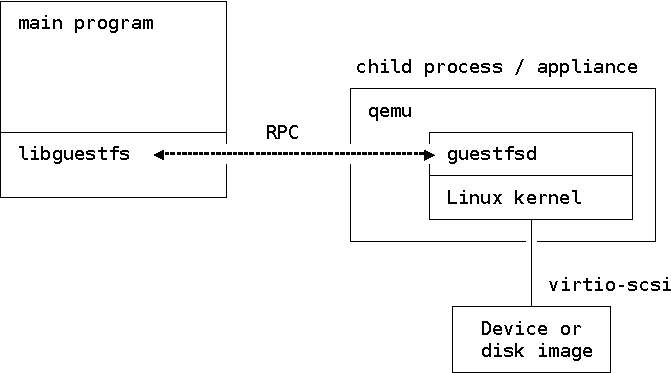
\includegraphics[width=.65\textwidth]{frames/img/libguestfs_arch}
\end{center}
    
    \note{
        \begin{itemize}
            \item \textbf{Q} library and suite of utilities for offline FS access
            \item Approach: runs a small virtual machine with  Linux that does the FS-access
            \item process on the host talks to process in the VM
            \item quite some overhead, but the goal is to isolate the operations from the host
            \item fast CLI utils, slow FUSE => additional overhead, because data is transferred in smaller chunks
        \end{itemize}
    }
\end{frame}